\documentclass[a4paper,titlepage,oneside]{article}

\usepackage{amsmath}
\usepackage{amsfonts}
\usepackage{amssymb}
\usepackage{amsthm}
\usepackage[utf8]{inputenc}
\usepackage[T1]{fontenc}
\usepackage{enumitem}
\usepackage{ngerman}
\usepackage{mathtools}
\usepackage{tikz}
\usepackage{setspace}
\usepackage{geometry}

%Formatting
\author{Tanja Kohler}
\title{Analysis für Informatik\small{ \\ - \\ Ass.Prof. Clemens Amstler}}
\geometry{verbose,a4paper,tmargin=25mm,bmargin=25mm,lmargin=25mm,rmargin=25mm}

%Definitions
%Konstante Mengen und Zahlen C, N, Q Z, R, i, e
\def\C{\ensuremath{\mathbb{C}} }
\def\N{\ensuremath{\mathbb{N}} }
\def\Q{\ensuremath{\mathbb{Q}} }
\def\Z{\ensuremath{\mathbb{Z}} }
\def\R{\ensuremath{\mathbb{R}} }
\def\im{\ensuremath{\mathit{i}} }
\def\e{\ensuremath{\mathit{e}}}

% für Beweise
\def\WSP{\text{Widerspruch! }}
\newcommand{\IA}[1][n=0]{\vspace{0.1pt}\ensuremath{\text{IA}\sp#1:}}
\newcommand{\IV}{\vspace{0.1pt}\ensuremath{\text{IV}\sp}}
\newcommand{\IS}[1][n \mapsto n+1]{\vspace{0.1pt}\ensuremath{\text{IS}\sp#1}}

%Abkürzungen logischer symbole
\def\fa{\ensuremath{\forall}}
\def\ex{\ensuremath{\exists}}
\def\xor{\ensuremath{\veebar}}
\def\lor{\ensuremath{\vee}}
\def\land{\ensuremath{\wedge}}
\def\nand{\ensuremath{\not \land}}
\def\nor{\ensuremath{\not \lor}}

%spacing
\def\sp{\hspace{0,1cm}}

%infinite sums
\newcommand{\suminf}[2][n]{\ensuremath{\sum_{#1= 0}^{\infty}{#2}}}
\newcommand{\Suminf}[2][n]{\ensuremath{\sum_{#1=1}^{\infty}{#2}}}

% summe vereinfachen
\newcommand{\Sum}[2]{\sum_{#1}^{#2}}

% limits bis unendlich -unendlich und 0
\renewcommand{\liminf}[2][n]{\ensuremath{\lim\limits_{#1 \rightarrow \infty}{#2}}}
\newcommand{\limInf}[2][n]{\ensuremath{\lim\limits_{#1 \rightarrow -\infty}{#2}}}
\newcommand{\limnull}[2][n]{\ensuremath{\lim\limits_{#1 \rightarrow 0}{#2}}}

% limits von + nach 0 bzw von - nach 0
\newcommand{\limpos}[2][n]{\ensuremath{\lim\limits_{#1 \rightarrow 0^+}{#2}}}
\newcommand{\limneg}[2][n]{\ensuremath{\lim\limits_{#1 \rightarrow 0^-}{#2}}}

% absolutbetrag mit abständen zwischen | und inhalt.
\newcommand{\abs}[1]{\ensuremath{\left|\:#1\:\right|}}

% mathematische definitionen, menge, funktion
\newcommand{\menge}[2]{\ensuremath{\{#1\sp : \sp #2\}}}
\newcommand{\funktion}[3]{\ensuremath{#1: #2 \to #3}}
\newcommand{\Funktion}[5]{\ensuremath{#1: #2 \to #3 \text{ mit } #4 \mapsto #5}}

% konvergiert gegen inf 
\newcommand{\toinf}[1]{#1 \rightarrow \infty}
\newcommand{\longtoinf}[1][n]{\ensuremath{\overset{\scriptscriptstyle{#1 \to \infty}}{\longrightarrow}}}
\newcommand{\tonull}[1]{#1 \rightarrow 0}
\newcommand{\longtonull}[1][n]{\ensuremath{\overset{\scriptscriptstyle{#1 \to 0}}{\longrightarrow}}}
\newcommand{\toInf}[1]{#1 \rightarrow -\infty}
\newcommand{\longtoInf}[1][n]{\ensuremath{\overset{\scriptscriptstyle{#1 \to -\infty}}{\longrightarrow}}}

% Umgebungsstil, einer für alle
\newtheoremstyle{thmstyle}{}{0.5cm}{}{}{\bfseries}{}{\newline}{\thmnumber{#2. }\thmname{#1}\quad\thmnote{ #3}}

% umgebungen 
\theoremstyle{thmstyle}
\newtheorem{satz}{Satz}[subsection]
\newtheorem{korr}[satz]{Korollar}
\newtheorem{prop}[satz]{Proposition}
\newtheorem{defi}[satz]{Definition}
\newtheorem{bsp}[satz]{Beispiel}
\newtheorem{bem}[satz]{Bemerkung}

% beweis umgebung anpassen: anfang und ende
\renewcommand{\proofname}{\textbf{Beweis:}}
\renewcommand{\qedsymbol}{\textit{q.e.d.}}

%Documentstart
\begin{document}

\maketitle

\onehalfspace
\section{Reelle und Komplexe Zahlen}
\subsection{Reelle Zahlen}
Die reellen Zahlen \R erfüllen eine Reihe von Axiomen, die in drei Gruppen unterteilt werden können.

\begin{enumerate}[label=\Roman*.]
	\item Algebraische Axiome
	\item Anordnungsaxiome
	\item Vollständigkeitsaxiome
\end{enumerate}

\subsubsection{Algebraische Axiome}
Die reellen Zahlen bilden mit der Addition \( + : \R \times \R \to \R \text{ mit } (a,b) \mapsto a + b\) und der Multiplikation \( * :  \R \times \R \to \R \text{ mit } (a,b) \mapsto a * b \)
einen Körper \((\R, +, * )\), der folgende Axiome erfüllt: 
\begin{enumerate}[label=\arabic*)]
	\item \(\R\) ist bzgl. der Addition eine Abelsche Gruppe. \((\R,+)\)
	\item \(\R \setminus \{0\}\) ist bzgl der Multiplikation eine Abelsche Gruppe. \((\R,*)\)
	\item Das Distributivgesetz gilt: \( \fa a,b,c \in \R \sp a * (b + c) = a * b + a * c\)
\end{enumerate}
Andere Beispiele von Körpern: \C, \Q, \(\Z_p \text{ für }p\) prim.
Die Natürlichen Zahlen \(\N = \{1,\dots,\infty \} \) und die Ganzen Zahlen \Z bilden keinen Körper.

\begin{prop}
\(\fa x \in \R \text{ gilt } 0 * a = 0\).
\begin{proof}\begin{flalign*}0+0 = 0 	&\Rightarrow a ( 0 + 0 ) = a * 0 					&&\text{Distributivgesetz }\\
							& \Rightarrow a * 0 + a * 0 = a * 0 				&&\text{\R assiozativ}\\
							&\Rightarrow a * 0 + (a * 0 - a * 0) = (a * 0 - a * 0) 	&& \text{add Inv}\\
							&\Rightarrow a * 0 +  0	 					&& 0+0 = 0\\
							&\Rightarrow a * 0 = 0 \end{flalign*}
\end{proof}
\end{prop}

\begin{defi}[Potenzschreibweise]
Für \(a \in \R \text{ und }n \in \Z \text{ wird }a^n\) folgendermapen induktiv definiert:
\begin{itemize}
	\item \(a^0 = 1\)
	\item \(\fa n > 1 \quad a^{n+1} = a * a^n \)
	\item \(\fa n > 1 \sp \fa a \ne 0 \quad a^{-n} = \left(a^{-1}\right)^n\)
\end{itemize}
\end{defi}
\newpage

\begin{bem}
\(\fa a, b \in \R \setminus \{0\} \) und \( \fa n, m \in \Z\) gilt:
\begin{enumerate}[label=(\arabic*)]
	\item $\displaystyle a^n * a^m = a^{n+m} $
	\item $\displaystyle a^{n^m} = a^{n * m} $
	\item $\displaystyle a^n * b^n = (a * b)^n $
\end{enumerate}
\begin{proof}\sp
\begin{enumerate}[label=(\arabic*)]
	\item $\displaystyle a^n * a^m \overset{\text{n. Def.}}{=} \overbrace{a \dots a}^{n\text{-mal}}*\overbrace{a \dots a}^{m\text{-mal}} = \overbrace{a \dots a}^{n+m\text{-mal}} \overset{\text{n. Def.}}{=} a^{n+m}$
	\item $\displaystyle a^{n^m} = a^{\overbrace{n \dots n}^{m\text{-mal}}} = a^{m * n} = a^{n*m}$
	\item $\displaystyle a^n * b^n = \overbrace{a \dots a}^{n\text{-mal}}*\overbrace{b \dots b}^{n\text{-mal}} = \overbrace{a \dots a b \dots b}^{n\text{-mal}} = (a*b)^{n}$
\end{enumerate}
\end{proof}
\end{bem}

\subsubsection{Anordnungsaxiome}
Die reellen Zahlen werden in positive Zahlen, negative Zahlen und 0 unterteilt. Dabei ist \(x < 0 \Leftrightarrow -x > 0\) Und es gelten folgende Axiome:
\begin{enumerate}[label=(\arabic*)]
	\item \(\fa x \in \R \) gilt genau eine der folgenden Bedingungen: \(x > 0\text{, } x = 0\text{, } x < 0 \)
	\item \(\fa x,b \in \R \sp x,b > 0 \text{ gilt: } a + b > 0 \land a * b > 0\)
\end{enumerate}
Wir schreiben für \(a, b \in \R \sp a > b \Leftrightarrow a - b > 0\text{ und }a \ge b \Leftrightarrow a > b \lor a = b \)

\begin{prop}
\(\fa a, b \in \R \) gilt: \(a < b \text{ und } b < c \Rightarrow a < c\)
\begin{proof}
Sei \( a < b \text{ und } b < c \Rightarrow a - b < 0  \text{ und } b - c < 0 \Rightarrow a - b + b - c < 0 \Rightarrow a - c < 0 \Rightarrow a < c\)
\end{proof}
\end{prop}

\begin{bem}
\(\fa a, b, c \in \R\) gilt:
\begin{enumerate}[label=\alph*)]
	\item \(a < b \Rightarrow a + c < b + c\)
	\item \(a < b \text{ und } c > 0 \Rightarrow a * c < b * c\)
	\item \(a < b \text{ und } c < 0 \Rightarrow a * c > b * c\)
	\item \(a \ne 0 \Rightarrow a^2 > 0 \text{ speziell } 1 > 0\)
	\item \(0 < a < b \text{ und } a < b < 1 \Rightarrow b^{-1} < a^{-1}\)
\end{enumerate}
\end{bem}

\begin{defi}
Für \(a \in \R\) und der Betrag \abs{a} folgendermaßen definiert. 
\[\abs{a} = \begin{cases}
		 a 	& a > 0\\
		-a 	& a < 0  \end{cases}\]
\end{defi}

\newpage
\begin{satz}
\(\fa b \in \R\) gilt:
\begin{enumerate}[label=(\arabic*)]
	\item \(\abs{a * b} = \abs{a} * \abs{b}\)
	\item \(\abs{a + b} \le \abs{a} + \abs{b}\) (Dreiecksungleichung)
	\item \(\abs{a - b} \ge \abs{\abs{a} - \abs{b}}\) (umgekehrte Dreiecksungleichung)
\end{enumerate}
\begin{proof}\sp
\begin{enumerate}[label=(\arabic*)]
	\item Beweis durch Falltunterscheidung.
	\item \begin{itemize}
		\item \(\quad a \le \abs{a} \text{ und } \sp \quad b \le \abs{b} \quad \Rightarrow \quad a + \quad b \quad\le\quad \abs{a}+\abs{b} \) 
		\item \(\sp-a \le \abs{a} \text{ und } -b \le \abs{b} \quad \Rightarrow \sp -a + \sp -b \quad\le\quad \abs{a} +\abs{b} \)
		\end{itemize}
		\(\Rightarrow a + b \le \abs{a} + \abs{b} \text{ und } -(a + b) \le \abs{a} + \abs{b} \Rightarrow \abs{a + b} \le \abs{a} + \abs{b} \)
	\item \begin{itemize}
		\item \(\abs{a} = \abs{a - b + b} \le \abs{a - b} + \abs{b} \Rightarrow \abs{a} - \abs{b} \le \abs{a-b}\)
		\item \(\abs{b} = \abs{a - b - a} \le \abs{a - b} + \abs{a} \Rightarrow \abs{b} - \abs{a} \le \abs{a-b}\)
		\end{itemize}
		\(\Rightarrow \abs{a} - \abs{b} \le \abs{a-b} \text{ und } - (\abs{a} - \abs{b}) \le \abs{a-b} \\
	\Rightarrow \abs{\abs{a} - \abs{b}} \le \abs{a-b}\)
\end{enumerate}
\end{proof}
\end{satz}

\begin{bem}[Archimedisches Axiom]
Für zwei positive Zahlen, \(a, b\) gibt es immer eine natürliche Zahl $n$, sodass folgendes gilt: \(n * b > a\) Also:
\[\fa a,b > 0 \sp \ex n \in \N \quad n * b > a\]
Als Folgerung erhalten wir: Setze \(b = 1\)
\[\fa a > 0 \sp \ex n \in \N \quad n > a\]
\end{bem}

\begin{satz}[Bernoullische Ungleichung]
Sei \(a > -1\) dann gilt \[\fa n \in \N \sp (1+a)^n \ge 1 + na \]
\begin{proof}
\begin{math}
\begin{aligned}[t]
	&\IA{n=0} \sp 1 = (1 + a)^0 \ge 1 + 0*a = 1				&&\\
	&\IV (1+a)^n \ge 1 + na								&&\\
	&\IS{n \mapsto n+1} \\ 
	&\begin{aligned}[t]
		(1+a)^{n+1} 	&= (1+a)(1+a)^n 					&&\\
					&\overset{IV}{\ge} (1 + a)(1 + na) 		&&\\
					&= 1 + na + a + \underbrace{na^2}_{> 0} 	&&\\
					&\ge 1 + (n+1)a \end{aligned}
\end{aligned}
\end{math}
\newline
\end{proof}
\end{satz}
\newpage

\begin{korr}
Sei \(a > 0\).
\begin{enumerate}[label=(\arabic*)]
	\item Ist \sp \(a > 1 \sp \forall k > 0 \sp \exists n \in \N \text{, sodass }a^n > k.\)
	\item \(0 < a < 1 \sp \forall \epsilon > 0 \sp \exists n \in \N \text{, sodass }a^n < \epsilon\)
\end{enumerate}
\begin{proof}\sp
\begin{enumerate}[label=(\arabic*)]
	\item \begin{math}
		\text{Sei } a = x + 1 > 1 \Rightarrow a^n = (x + 1)^n \overset{\text{Bernoulli}}{\ge} 1 + nx \\
		\forall n \in \N \sp \exists x > 0 \text{ mit } nx > k - 1 \Rightarrow a^n \ge 1 + nx > 1 + k -1 = k 
		\end{math}
	\item \begin{math}
		\text{Sei } 0 < a < 1 \text{ und } b = \frac{1}{a} > 1 \overset{\tiny{mit (1)}}{\Rightarrow} \exists k \in \R \text{ mit }  \left(\frac{1}{a}\right)^n = b^n > k = \frac{1}{\epsilon}\\
		\Rightarrow  \left(\frac{1}{a}\right)^n > \frac{1}{\epsilon} \Rightarrow  \frac{1}{a^n} > \frac{1}{\epsilon} \Rightarrow a^n < \epsilon.
		\end{math}
\end{enumerate}
\end{proof}
\end{korr}

\subsubsection{Vollständigkeitsaxiom}
Die Zahlengerade \R hat keine Lücken. 

\begin{defi}
Sei \(M \subset \R\) eine Teilmenge.
\begin{enumerate}
	\item \(k \in \R\) heißt obere Schranke von \(M\) wenn gilt, \(\fa x \in M,\sp x \le k\). \(M\) heißt nach oben beschränkt, 
		wenn es eine obere Schranke gibt. zB \N ist nicht nach oben beskchränkt, nach dem Archimedischem Axiom.
	\item \(k \in \R \) heißt untere Schranke von \(M\) wenn gilt, \(\fa x \in M,\sp x \ge k\). \(M\) heißt nach unten beschränkt, 
		wenn es eine untere Schranke gibt.
	\item \(M\) heißt beschränkt, wenn eine obere und untere Schranke existiert.  Äquivalente Definition für Beschränktheit: 
		\(\exists k \in \R,\sp \abs{x} \le k \sp \fa x \in M\)
	\item \(a \in \R\) heißt Infimum von \(M\), falls \(a\) größte untere Schranke von \(M\) ist. Das heißt \(a\) ist untere Schranke 
		von \(M\) und ist \(k\) eine untere schranke von \(M\), dann folgt \(k \le a\)
		\[\text{Schreibweise: } a = inf(M)\]
	\item \(b \in \R\) heißt Supremum von \(M\), falls \(b\) kleinste obere Schranke von \(M\) ist. Das heißt \(b\) ist obere 
		Schranke von \(M\) und ist \(k\) eine obere schranke von \(M\), dann folgt \(k \ge a\) \[\text{Schreibweise: } b = sup(M)\]
\end{enumerate}
\end{defi}

\begin{bsp}
Sei \(a < b\) dann ist \(inf[a,b] = a = inf(a,b) \text{ und } sup[a,b] = b = sup(a,b)\).
\begin{align*}
[a, b] = &\sp \menge{a \in \R}{a \le x \le b} \sp \text{ heißt abgeschlossenes Intervall}\\
(a, b) = &\sp \menge{a \in \R}{a < x < b} \sp \text{ heißt offenes Intervall}
\end{align*}
\end{bsp}

\begin{bem}[zur Erinnerung]
Definition der natürlichen Zahlen (Axiom des kleinsten Element (Pianoaxiome)) \\
Jede Teilmenge der natürlichen Zahlen hat ein kleinstes Element.
\end{bem}

\begin{satz}[Vollständigkeitsaxiom]
Jede nicht leere, nach unten beschränkte Teilmenge \(M \subset \R\)  besitzt ein Infimum \(inf(M) \in \R\).
\proof[ohne Beweis]
\end{satz}

\begin{bem}
\(inf(M)\) muss kein Element von \(M\) sein.
\end{bem}

\begin{prop}
Jede nicht leere nach oben bescrhänkte Teilmenge \(M \subset \R\) besitzt ein Supremum \(sup(M) \in \R\).
\begin{proof}
Seien \(M\) nach oben beschränkt und \(a\) eine obere Schranke von \(M\).\\
\(\Rightarrow \fa x \in M  \quad x \le a \Rightarrow -a \le -x \quad \fa x \in M \Rightarrow -a\) ist untere Schranke von \(-M = \menge{-x}{x \in M}\\
\Rightarrow -M\) ist nach unten beschränkt. Nach dem Vollständigkeitsaxiom, existiert ein Infimum.\\
Sei \(b= inf(-M) \Rightarrow -a \le b \Rightarrow -b \le a \text{ und } b \le -x \Rightarrow x \le -b \quad \forall x \in M\).\\
Also \(-b\) ist obere Schranke und kleinste obere Schanke. \(\Rightarrow -b = sup(M)\)
\end{proof}
\end{prop}

\begin{prop}
\(sup(M) \text{ und } inf(M)\) sind eindeutig bestimmt.
\begin{proof}
Seien \(m\) und \(m'\) Suprema von \(M \Rightarrow m \le m' \text{ und } m' \le m \Rightarrow m = m'\).\\
analog für Infimum.
\end{proof}
\end{prop}

\subsection{Komplexe Zahlen}
Die Menge der komplexen Zahlen \C sind die Punkte der Ebene \(\R^2 = \{(a,b) : a,b \in \R\}\)
\[(a,b) = (a, 0) + (0, b) = a (1,0) + b (0, 1)\]
Wir setzen \(1 = (1,0), \im = (0,1) \Rightarrow z = (a, b) = a + \im b\)\\
\begin{center}
\begin{tikzpicture}
        \draw[step=1,help lines,black!0] (-1,-1) grid (4,4);
        \draw[->] (-0.5,0) -- (3.5,0)  node[below right] {$Re(z)$};
        \draw[->] (0,-0.5) -- (0,3.5)  node[above left]{$Im(z)$};
        \draw[-] (2.21,1.75) -- (2.21,0) ;
        \draw[-] (2.21,1.75) -- (0,1.75) ;
        \foreach \Point/\PointLabel in {(0,1)/{\im}, (1,0)/1, (2.21,1.75)/{z=(a,b)}}
        \draw[fill=black] \Point circle (0.05) node[above right] {$\PointLabel$};
        \foreach \Point/\PointLabel in {(2.21,0)/a, (0,1.75)/b}
        \draw \Point circle (0.05) node[above right] {$\PointLabel$};
\end{tikzpicture}
\end{center}
zusätzlkich verlangen wir \(\im^2 = -1\) Also: \(\C = \menge{z = a + \im b }{ a, b \in \R, \im^2 = -1 }\)

\newpage
\begin{satz}
Es gilt:  \C ist ein Körper.
\begin{proof} Sei \( x,y,z \in \C \text{ und } x = a + \im b, y = c + \im d, z = e + \im f \)
\begin{enumerate}[label=\Roman*)]
\item \C ist eine abelsche Gruppe bezüglich der Addition:
\begin{enumerate}[label=\roman*)]
\item \( x + y = a + \im b + c + \im d = (a+c) + \im (b + d) \in \C\)
\item \(x + 0 = a + \im b + 0 + \im 0 = a + \im b = x \)
\item \( \exists -x \in \C \text{ mit } x + -x = a + \im b - a -\im b = 0 \)
\item \( x+y =  (a+c) + \im (b + d) =  (c + a) + \im (d + b) = y + x \)
\end{enumerate}
\item \C ist eine abelsche Gruppe bezüglich der Multiplikation:
\begin{enumerate}[label=\roman*)]
\item \( xy = (a + \im b)(c + \im d) = (ac - bd) + \im (ad - bc) \in \C\)
\item \( 1x = (1+\im 0)(a + \im b ) = a + \im b = x \)
\item \( \exists x^{-1} \in \C \text{ mit } xx^{-1} = (a + \im b)\frac{a + \im b}{a^2 - b^2} = \frac{a^2 - b^2}{a^2 - b^2} = 1\)
\item \( xy = (ac - bd) + \im (ad - bc) = (ca - bd) + \im (da - cb) = yx\)
\end{enumerate}
\item Das Distributivgesetz gilt:\\
 \begin{math}\begin{aligned} z (x + y) &= (e + \im f)( a+c + \im b + \im d) \\
 &= ea + ec - fb - fd + \im fa +\im fc + \im eb + \im ed \\
 &= ea - fb + \im fa + \im eb + ec - fd + \im ed + \im fc \\
 &= xy + xz\end{aligned}\end{math}
\end{enumerate}
\end{proof}
\end{satz}

\begin{defi}
Sei \( z = a + \im b \in \C \)
\begin{itemize}
\item \(\overline{z} = a - \im b \) heißt die konjungiert komplexe Zahl von $z$.
\item \(\abs{z} = \sqrt{z \overline{z}} = \sqrt{a^2 + b^2}\) heißt Betrag von \(z\).
\item $a = Re(z)$ heißt Realteil von $z$.
\item $b = Im(z)$ heißt Imaginärteil von $z$.
\end{itemize}
\end{defi}

\newpage
\begin{satz}
Es gilt: \[Re(z) = \frac{z + \overline{z}}{2} \text{ und } Im(z) = \frac{z - \overline{z}}{2\im}\]
\begin{proof} \sp
\begin{center}
\begin{tikzpicture}
        \draw[step=1,help lines,black!0] (-1,-2.5) grid (4,3);
        \draw[<->] (-0.5,0) -- (3.5,0)  node[below right] {$Re$};
        \draw[<->] (0,-2) -- (0,2.5)  node[above left]{$Im$};
        \draw[-] (1.5,1) -- (1.5,0) ;
        \draw[-] (1.5,1) -- (0,1) ;
        \draw[fill=black] (1.5,1) circle (0.05) node[above] {$\scriptstyle z$};
        \foreach \Point/\PointLabel in {(1.5,-1)/\overline{z}, (3, 0)/{z+\overline{z}}, (1.5,0)/{\frac{z+\overline{z}}{2} = Re(z)}}
        \draw[fill=black] \Point circle (0.05) node[below] {$\scriptstyle \PointLabel$};
         \foreach \Point/\PointLabel in {(0,2)/{z-\overline{z}}, (0,1)/{Im(z) = \frac{z-\overline{z}}{2\im}}}
        \draw[fill=black] \Point circle (0.05) node[left] {$\scriptstyle \PointLabel$};
\end{tikzpicture}
\end{center}
\end{proof}
\end{satz}

\begin{prop}
Es gilt:
\begin{enumerate}[label=(\roman*)]
\item \( \overline{\overline{z}} = z, \quad \overline{z_1} + \overline{z_2} = \overline{z_1 + z_2}, \quad \overline{z_1}* \overline{z_2} = \overline{z_1  z_2}, \quad \abs{\overline{z}} = \abs{z} \)
\item \( \abs{z} \ge 0, \quad \abs{z} = 0 \Leftrightarrow z = 0\)
\item \(\abs{z_1 z_2} = \abs{z_1} \abs{z_2}\)
\item \(\abs{z_1 + z_2} \le \abs{z_1} + \abs{z_2}\)
\end{enumerate}
\begin{proof} \sp
\begin{enumerate}[label=(\roman*)]
\item
\begin{itemize}
\item \(\overline{\overline{z}} = \overline{\overline{a + \im b}} = \overline{a - \im b} = a + \im b = z \)
\item \(\overline{z_1} + \overline{z_2} = a - \im b + c - \im d = (a + c) - \im (b + d) = \overline{z_1 + z_2} \)
\item \(\overline{z_1} * \overline{z_2} = (a - \im b) (c - \im d) = (ac + bd) - \im (ac + bc) = \overline{z_1  z_2} \)
\item \( \abs{\overline{z}} = \sqrt{a^2 + b^2} = \abs{z}\)
\end{itemize}
\item
\begin{itemize}
\item \(\abs{z} = a^2 + b^2 > 0 \)
\item \(\abs{z} = a^2 + b^2 = 0 \Leftrightarrow a^2 = - b^2 \Leftrightarrow a = b = 0 \)
\end{itemize}
\item \(\abs{z_1 z_2}^2 = (z_1 z_2)(\overline{z_1 z_2}) = (z_1\overline{z_1})(z_2\overline{z_2}) = \abs{z_1}^2\abs{z_2}^2 \Leftrightarrow \abs{z_1 z_2} = \abs{z_1}\abs{z_2} \) 
\item  \begin{math}  
\text{Sei }a, b \in \R \sp z \in \C \sp z = a + \im b \\
\begin{aligned}[t]
Re(z)^2 = a^2 \le a^2 + b^2 = \abs{z}^2 &\Rightarrow Re(z) \le \abs{Re(z)} = \sqrt{Re(z)} \le \abs{z} \\
&\Rightarrow Re(z_1\overline{z_2}) \le \abs{z_1\overline{z_2}} = \abs{z_1}\abs{\overline{z_2}} = \abs{z_1}\abs{z_2} \\
\end{aligned}\\
\begin{aligned}[t]
\abs{z_1 + z_2}^2 &= (z_1 + z_2)\overline{(z_1 + z_2)} = (z_1 + z_2)(\overline{z_1} + \overline{z_2}) \\
&= z_1\overline{z_1} + z_2\overline{z_1} + z_1\overline{z_2} + z_2\overline{z_2} &&\text{denn } z_2\overline{z_1} = \overline{z_1\overline{z_2}} \\
&= \abs{z_1}^2 + z_1\overline{z_2} + \overline{z_1\overline{z_2}} + \abs{z_2}^2 &&\text{denn } z_1\overline{z_2} + \overline{z_1\overline{z_2}} = 2Re(z_1z_2) \\
&= \abs{z_1}^2 + 2 Re(z1 \overline{z2}) + \abs{z_2}^2 &&\text{denn } Re(z_1z_2) \le \abs{z_1}\abs{z_2}\\
&\le  \abs{z_1}^2 + 2\abs{z_1}\abs{z_2} + \abs{z_2}^2 = \left(\abs{z_1} + \abs{z_2}\right)^2
\end{aligned}\\
\Rightarrow \abs{z_1 + z_2} \le \abs{z_1} + \abs{z_2}
\end{math}  
\end{enumerate}
\end{proof}
\end{prop}

\section{Folgen und Reihen}
\subsection{Folgen}

\begin{bsp} 
Betrachte 
\begin{center} 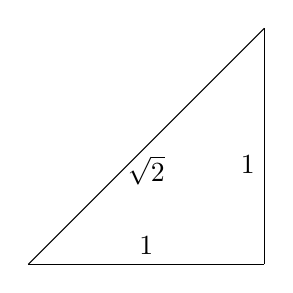
\begin{tikzpicture}[scale=3]
 \draw (0,0) -- node[above] {$1$} (1,0);
 \draw (1,0) -- node[below left] {$1$} (1,1);
 \draw (0,0) -- node[below] {$\sqrt{2}$}  (1,1);
 \end{tikzpicture} \end{center}
Annahme: \( \sqrt{2} \in \R\), aber \(\sqrt{2} \not\in \Q\)
\end{bsp}
\begin{proof} Angenommen $\displaystyle \sqrt{2} \in \Q$ \\
$ \displaystyle \sqrt{2} \in \Q \Rightarrow \frac{p}{q} \text{ mit }p \in \Z, q \in \N $ und p und q nicht beide durch 2 teilbar, sonst kürzen wir.
\begin{align*}
2 &= \frac{p^2}{q^2} &\Rightarrow\\
2q^2 &= p^2 &\Rightarrow &&\text{Also } 2 | p^2 \Rightarrow 2 | p \Rightarrow \exists m \text{ mit } p = 2 m. \\
2q^2 &= (2m)^2 = 4m^2 &\Rightarrow \\
q^2 &= 2m^2 & &&\text{ d.h. } 2 | q^2 \Rightarrow 2 | q \text{ Also p und q sind beide durch 2 teilbar.}
\end{align*}
 \WSP p und q sind nicht beide durch 2 teilbar. $\displaystyle \Rightarrow \sqrt{2} \not\in \Q \Rightarrow \sqrt{2} \in \R\setminus\Q$
\end{proof}

\begin{bem}
\( \sqrt{2} \) ist die positive Lösung von $ \displaystyle a^2 = 2 \Leftrightarrow a = \frac{2}{a} \Leftrightarrow  2a = a + \frac{2}{a} \Leftrightarrow a= \frac{1}{2}\left(a + \frac{2}{a}\right)$ \\
Betrachte die rechte Seite dieser Gleichung und berechne diese induktiv\\
Setze zB
\begin{align*}
a_1 &= 1\\
a_{n+1} &= \frac{1}{2}\left(a_n + \frac{2}{a_n}\right)
\end{align*}
\begin{align*}
a_1 = 1 && a_2 = 1,5 && a_3 \approx 1.41 && a_3 \approx 1,4142 &&\dots 
\end{align*}
Also \(a_n\) nähert sich mit wachsendem \(n\) immer mehr an \(\sqrt{2}\). Dies führt zu dem Begriff \textbf{Grenzwert einer Folge}.
\end{bem}

\begin{defi}
Eine Folge $(a_n)_{k=0}^{\infty}$ reeller Zahlen ist eine Abbildung $\N_0 \rightarrow \R\text{ mit } n \mapsto a_n$ 
Bezeichnung: Wir schreiben für Folgen
\begin{align*}
&(a_n)_{k=0}^{\infty} && (a_n)_{n\ge0} && (a_n)_{n\in\N} & (a_n) && (a_n)_{n\ge n_0} 
\end{align*}
\end{defi}

\newpage
\begin{defi}
Eine Folge \((a_n)\) heißt 
\begin{enumerate}
\item (streng) monoton wachsend, wenn \( \fa a \in \N \sp a_n \le a_{n+1}	\quad (a_n)\nearrow	\quad (a_n < a_{n+1} \quad (a_n)\uparrow)\)
\item (streng) monoton fallend, wenn \( \fa a \in \N \sp a_n \ge a_{n+1}	\quad (a_n)\searrow	\quad (a_n > a_{n+1} \quad (a_n)\downarrow)\)
\item (streng) monoton, sie (streng) monoton wachsend oder (streng) monoton fallend ist.
\end{enumerate}
\end{defi}

\begin{bsp}
Ein paar Beispiele zu Folgen:
\begin{enumerate}[label=(\arabic*)]
\item Die konstante Folge \(a_n = k\) ist monoton fallend und steigend.
\item Die harmonische Folge $ \displaystyle a_n = \frac{1}{n} \sp \fa n \ge 1$ ist streng monoton fallend.
\item Die alternierende Folge $ \displaystyle a_n = (-1)^n $ ist nicht monoton.
\item Die geometische Folge $ \displaystyle  a_n = a^n \sp \fa n \ge 0 $ Sei $ \displaystyle a \in \R \sp a^n \text{ ist } 
				\begin{cases}			\text{streng monoton wachsend} 	& a > 0\\
									\text{streng monoton fallend} 		& 0 < a < 1\\
									\text{monoton} 					& a = 1\\
									\text{nicht monoton} 				&  \end{cases} $
\item Die Fibonacci Folge ist monoton wachsend. $ \displaystyle f_n = \begin{cases}	1				& \text{wenn } n = 0, n = 1\\
																f_{n-1} + f_{n-2}	& \text{sonst} \end{cases} $
\end{enumerate}
\end{bsp}

\begin{defi}[der Konvergenz]
Eine Folge reeller Zahlen \((a_n)_{n\in\N}\) heißt konvergent gegen \( a\in\R\) wenn 
\[\forall \epsilon > 0 \quad \exists N \in \N \quad \forall n \ge N \quad \abs{a_n - a} < \epsilon\]
\(a\) heißt der Grenzwert oder Limes der Folge \((a_n)\). Die Folge \((a_n)\) heißt divergent, wenn sie nicht konvergiert. Schreibweise: \(\lim{a_n} = a \) oder \( \lim\limits_{n \to k}{a_n} = a \). Wobei \( k \in \R\cup\{\infty, -\infty\}\)
\end{defi}

\begin{bem}
Sei \(a \in \R, \epsilon > 0\). \(U_\epsilon(a) = (a-\epsilon, a+\epsilon) = \menge{x \in \R}{a - \epsilon < x < a + \epsilon} \text{ heißt } \epsilon\text{-Umgebung von }a\).
\[ a_n \in U_\epsilon(a) \Leftrightarrow a-\epsilon < a_n < a + \epsilon \Leftrightarrow -\epsilon < a_n - a < \epsilon \Leftrightarrow \abs{a_n - a} < \epsilon\]
Also: Die Folge \((a_n)\) konvergiert gegen \(a \Leftrightarrow \) Die Folgenglieder \(a_n\) liegen ab einer Schwelle \(N\) alle in der \(\epsilon\)-Umgebung von \(a\). \((a_n)\) konvergiert nicht gegen \(a \Leftrightarrow \exists \epsilon > 0 \forall N\in\N \sp \exists n \ge N \abs{a_n - a} \ge \epsilon\).
\end{bem}

\newpage
\begin{bsp}
Beispiele zur Konvergenz:
\begin{enumerate}[label=(\arabic*)]
	\item Die harmonische Folge konvergiert: $ \displaystyle a_n = \frac{1}{n} \Rightarrow \liminf{\frac{1}{n}} = 0$
	\begin{proof}
		Sei $ \displaystyle \epsilon > 0 \text{ und } N > \frac{1}{\epsilon} \qquad \abs{a_n - 0} = \abs{\frac{1}{n} - 0} = \frac{1}{n} \le \frac{1}{N} < \epsilon $
	\end{proof}
	\item Die alternierende Folge $ \displaystyle b_n = (-1)^n$ ist divergent
	\begin{proof}
		Angenommen $ \displaystyle \exists a \in \R \text{ mit } \liminf{b_n} = b \\
		\text{Wähle } \epsilon = \frac{1}{2} > 0 \Rightarrow \exists N \in \N \sp \forall n \ge N \abs{b_n - b} < \frac{1}{2} \text{. Da } b_{n+1} - b_n = 		\pm 2 \text{ ist } \forall n \ge N \\ 
		\vphantom{\frac{1}{2}}\ 2 = \abs{b_{n+1} - b_{n}} = \abs{b_{n+1} - b - (b_n - b)} \le \abs{b_{b+1} - b} + \abs{b_n - b} < \frac{1}{2} + \frac{1}{2} = 1 \Rightarrow 2 < 1 \\
		\WSP \Rightarrow (b_n) $ ist divergent.
	\end{proof}
	\item Ob die geometsiche Folge \((a^n)_{n\ge1}\) hängt davon ab, welchen Wert $a$ hat.
	\begin{proof} Durch Fallunterscheidung
		\begin{enumerate}
			\item[Fall 1] \(\abs{a} < 1 \Rightarrow \liminf{a^n} = 0\) \\
				Sei \(\epsilon > 0 \overset{\text{Archimedisches Axiom}}{\Rightarrow} \sp \exists N \in \N \quad \abs{a}^N < \epsilon \Rightarrow \forall n \ge N \quad\abs{a^n - 0} = \abs{a}^n \le \abs{a}^N < \epsilon\)
			\item[Fall 2] \(a =  1 \Rightarrow a^n = 1 \Rightarrow \lim{a^n} = 1\)
			\item[Fall 3] \(a = -1 \Rightarrow \) divergent weil alternierend.
			\item[Fall 4] \(\abs{a} > 1 \quad  \forall K > 0 \sp \exists n \in \N \quad \abs{a}^n > K \text{ d.h. } (a^n)\) ist unbeschränkt.
		\end{enumerate}
	\end{proof}
\end{enumerate}
\end{bsp}

\begin{defi}
Eine Folge \((a_n)\) heißt nach oben (unten) beschränkt, wenn es ein \(A \in \R\) gibt mit \[\forall n \in \N \quad a_n \le A \qquad (a_n \ge A)\]
\((a_n)\) heißt beschränkt, wenn \((a_n)\) nach oben oder unten beschränkt ist. d.h. \[\exists K \in \R \quad \abs{a_n} \le K \lor \abs{a_n} \ge K \quad \forall n \in \N \]
\end{defi}

\begin{satz}
Jede konvergente Folge \((a_n)\) ist beschränkt.
\begin{proof}
\begin{math} \displaystyle
\begin{aligned}[t]
	&\liminf{a_n} = a. \quad \text{Wähle } \epsilon = 1 > 0 \Rightarrow \exists N \in \N \quad \forall n \ge N \quad \abs{a_n - a} < 1. \\
	&\abs{a_n} = \abs{a + (a_n - a)} \le \abs{a} + \abs{a_n- a} < \abs{a} + 1 \quad \forall n \ge N \\
	&\text{Sei } K = max\{\abs{a_1}, \abs{a_2}, \dots, \abs{a_{n-1}}, \abs{a}+1\} \\
	&\abs{a_n} < K \quad \forall n \ge 1 \\
\end{aligned}
\end{math}
\end{proof}
\end{satz}

\begin{bem}
Die Umkehrung gilt nicht. Das heißt eine beschränkte Folge ist nicht konvergent.\\
\textit{Gegenbeispiel}: die alternierende Folge $(-1)^n$.
\end{bem}

\begin{satz}[Monotoniekriterium]
Sei $(a_n)$ eine Folge. Dann gilt: 
\begin{itemize}
\item Ist $(a_n)$ monoton wachsend und nach oben beschränkt, dann ist $(a_n)$ konvergent.
\item Ist $(a_n)$ monoton fallend  und nach unten beschränkt, dann ist $(a_n)$ konvergent.
\end{itemize}
\begin{proof}
Es reicht die erste Aussage zu zeigen, denn ist $(a_n)$ monoton fallend und nach unten beschränkt \( \Rightarrow (-a_n)\) ist monoton wachsend und nach oben beschränkt $\Rightarrow (a_n) $ ist konvergent.

Sei also \((a_n) \nearrow \) und nach oben beschränkt. Mit dem Vollständigkeitsaxiom \(\Rightarrow \exists a = sup\menge{a_n}{n \in \N}\). Und sei $\epsilon > 0$ 
\begin{math}
\Rightarrow a - \epsilon \text{ ist keine obere Schranke von } \menge{a_n}{n \in \N} \Rightarrow \exists N \in \N \quad a-\epsilon < a_N \le a.\\
\text{Da }(a_n) \nearrow \begin{aligned}[t] 
					&\Rightarrow \forall n \ge N 						&& a_N \le a_n \\
					&\Rightarrow a-\epsilon < a_N \le a_n \le a < a+\epsilon 	&& \forall n \ge N \\
					&\Rightarrow a-\epsilon < a_n < a+\epsilon 			&& \forall n \ge N \\
					&\Rightarrow \abs{a_n - a} < \epsilon					&& \forall n \ge N \\
					&\Rightarrow \liminf{a_n} = a \end{aligned}\end{math}
\end{proof}
\end{satz}

\begin{bem}
Das Monotonie-Kriterium ist äquivalent zur Vollständigkeit.
\end{bem}

\begin{satz}
Der Grenzwert einer Folge ist eindeutig bestimmt.
\end{satz}
\begin{proof}
\begin{math} \displaystyle 
\text{Angenommen } \liminf{a_n} = a\text{ und }\liminf{a_n} = b\text{ und } a \ne b.\\
\text{Sei }\epsilon = \frac{1}{2}\abs{b-a} \begin{aligned}[t]
								&\Rightarrow \exists N_1 \sp \forall n \ge N_1 \sp \abs{a_n - a} < \epsilon \\
								&\Rightarrow \exists N_2 \sp \forall n \ge N_2 \sp \abs{a_n - b} < \epsilon \end{aligned}\\
\text{Sei } N = max\{N_1, N_2\} \quad \forall n \ge N \quad 
\begin{aligned}[t]
\abs{b-a} 	&= \abs{(b-a_n) + (a_n - a)} \\
		&\le \abs{b - a_n} + \abs{a_n - a} \\
		&= \abs{a_n - b} + \abs{a_n - a} \\
		&< \frac{1}{2}\abs{b-a} + \frac{1}{2}\abs{b-a} \\
		&= \abs{b-a}\\
\end{aligned}\\
\Rightarrow \abs{b-a}  < \abs{b-a} \WSP \Rightarrow a = b
\end{math}
\end{proof}

%% KORRIGIERE AB HIER!!
\begin{satz}[Rechenregeln für konvergente Folgen]
Seien \((a_n)\) und \((b_n)\) zwei konvergente Folgen. Dann gilt:
\begin{enumerate}
\item \((a_n \pm b_n)\text{ ist konvergent und }\liminf{a_n  \pm  b_n} = \liminf{a_n}  \pm \liminf{b_n}\).
\item \(\lambda (a_n)\text{ ist konvergent und }\liminf{\lambda a_n} = \lambda \liminf{a_n}\).
\item \((a_n b_n)\text{ ist konvergent und }\liminf{a_n b_n} = \liminf{a_n} \lim{n}{b_n}\).
\item Ist \((b_n) \ne 0 \sp \forall n \ge n_0\text{ und }\liminf{b_n} \ne 0\text{. Dann ist } \left(\frac{a_n}{b_n}\right) \text{ konvergent und }\liminf{\frac{a_n}{b_n}} = \frac{\liminf{a_n}}{\liminf{b_n}}\).
\item \(a_n \le b_n \text{ dann ist }\liminf{a_n} \le \liminf{b_n} \sp \forall n \ge n_0\).
\end{enumerate}
\begin{proof}
Sei \(\liminf{a_n} = 0\text{ und } \lim{b_n} = b\).
\begin{enumerate}
\item Sei $\epsilon > 0 \Rightarrow \exists N_1, N_2, \in \N \quad 
\begin{aligned}[t]
&\abs{a_n - a} < \frac{\epsilon}{2} \quad \forall n \ge N_1 \quad \text{ und } \quad  \abs{b_n - b} < \frac{\epsilon}{2} \quad \forall n \ge N_2\\
&\Rightarrow \forall n \ge max\{N_1, N_2\}\\
& \begin{aligned}[t]
\abs{(a_n \pm b_n) - (a \pm b)} &= \abs{(a_n - a) \pm (b_n - b)} \\
&\le \abs{a_n - a} + \abs{b_n - b} < \frac{\epsilon}{2} + \frac{\epsilon}{2} = \epsilon.
\end{aligned}\\
&\Rightarrow (a_n \pm b_n) \text{ beschränkt und } \liminf{a_n \pm b_n} = a+b.
\end{aligned}$
\item Sei $ \displaystyle \epsilon > 0 \Rightarrow \exists N \in \N \begin{aligned}[t] \quad 
		&\abs{a_n - a} < \frac{\epsilon}{\lambda} \quad \forall n \ge N\\
		& \abs{\lambda a_n - \lambda a} = \abs{\lambda(a_n - a)} = \abs{\lambda}\abs{a_n - a} < \lambda \frac{\epsilon}{\lambda} = \epsilon
		\end{aligned}$
\item Jede konvergente Folge ist beschränkt \(\Rightarrow \exists K \in \R \text{ mit } \abs{a_K} \le K \text{ und } \abs{b} \le K\\
Sei \epsilon > 0 \Rightarrow \exists N_1, N_2 \in \N \sp \abs{a_n - a} < \frac{\epsilon}{2K} \text{ und } \abs{b_n - b} < \frac{\epsilon}{2K}. \Rightarrow \forall n \ge max\{N_1, N_2\} \text{ gilt } \abs{a_n b_n - a b} = \abs{a_n b_n - a_n b + a_n b + a b} = \abs{ a_n (b_n - b) + b (a_n - a)} \le \abs{ a_n (b_n - b)} + \abs{b (a_n - a)} = \underbrace{\abs{a_n}}_{\le K} \abs{b_n - b} + \underbrace{\abs{b}}_{\le K}\abs{a_n - a} < K \frac{\epsilon}{2K} + K \frac{\epsilon}{2K} = \epsilon\)
\item 
Zeige \(\liminf{\frac{1}{b_n}} = \frac{1}{\liminf{b_n}}\\
\abs{\abs{ b_n } - \abs{b}} \le \abs{ b_n - b} < \frac{\abs{b}}{2} \sp \forall n \ge n_0 
\Rightarrow -\frac{\abs{b}}{2} < \abs{b_n} - \abs{b} < \frac{\abs{b}}{2}
\Rightarrow \frac{\abs{b}}{2} < \abs{b_n} \Rightarrow \frac{1}{\abs{b_n}} < \frac{2}{\abs{b}} \sp \forall n \ge n_0 
\text{Sei } \epsilon > 0 \Rightarrow \exists N \sp \forall n \ge N 
\abs{b_n - b} < \frac{\epsilon \abs{b} ^2}{2}
\Rightarrow \abs{\frac{1}{b_n} - \frac{1}{b}} = \abs{\frac{b - b_n}{b b_n}} = \frac{1}{\abs{b_n}}\frac{1}{\abs{b}} \abs{b - b_n} \text{  mit epsilon nach voraussetzungen abschätzen} \)  %TODO
\item 
Sei \(a_n \le b_n \forall n \ge n_0. zz. a \le b \)
Angenommen \(a > b\)
Sei \(\epsilon \frac{a-b}{2} > 0 \Rightarrow \exists N_1, N_2 \in \N \\
\abs{a_n - a} < \epsilon  \forall n \ge N_1 \\
\abs{b_n - b} < \epsilon  \forall n \ge N_2 \\
\Rightarrow \forall n \ge max\{N_1, N_2\} \\ 
b_n < b + \epsilon = b + \frac{a-b}{2} = \frac{2b + a - b}{2} = \frac{b + a}{2} = \frac{2a - a + b}{2} = a - \frac{a-b}{2} = a - \epsilon < a_n \\
\Rightarrow  b_n < a_n \forall n \ge max\{N_1, N_2\}  \WSP \Rightarrow a \le b \)
\end{enumerate}
\end{proof}
\end{satz}

\begin{satz}[Sandwich-Theorem]
Sei \((a_n)\text{ und }(b_n)\) zwei konvergente Folgen mit der Eigenschaft, dass \(\liminf{a_n} = \liminf{b_n} = a\).
Sei \((c_n)\) eine Folge mit der Eigenschaft, dass \(a_n \le c_n \le b_n \quad \forall n \ge n_0\)
Dann ist \((c_n)\) konvergent und \(\liminf{c_n} = a\).
\begin{proof}
\(\text{Sei }\epsilon > 0 \Rightarrow \exists  N_1, N_2 \in \N\)
\[a - \epsilon < a_n < a + \epsilon \quad \forall n \ge N_1\]
\[a - \epsilon < b_n < a + \epsilon \quad \forall n \ge N_2\]
\(\Rightarrow \forall n \ge max\{N_1, N_2\} 
\text{es gilt: } a-\epsilon < a_n \le c_n \le b_n < a + \epsilon \quad  \forall n \ge N
\Rightarrow \abs{c_n - a} < \epsilon \Rightarrow \liminf{c_n} = a\).
\end{proof}
\end{satz}

\begin{bsp}
\begin{enumerate}
\item Sei \((a_n)\) eine Folge mit \(0 \le a_n \le \frac{1}{n} \Rightarrow \liminf{a_n} = 0\)
\item \(a_n = \sqrt{2n} - \sqrt{n}\) ist divergent\\
denn \(a_n = \left(\sqrt{2n} - \sqrt{n}\right)\frac{\sqrt{2n} + \sqrt{n}}{\sqrt{2n} + \sqrt{n}} = \frac{2_n - n}{\sqrt{n}*\left(\sqrt{2} - 1\right)} \underbrace{\ge}_{\left(\sqrt{2} - 1\right)\le 3} \frac{n}{3\sqrt{n}} = \frac{sqrt{n}}{3} \longtoinf{n} \infty\).
\end{enumerate}
\end{bsp}

\begin{defi}
Eine Folge \((a_n)\) heißt bestimmt divergent gegen \(\pm \infty \) wenn gilt: \(\forall K \in \R \exists N \in \N \quad \forall n \ge N \sp a_n \lessgtr K \)
\[\text{Schreibweise: }\liminf{a_n} = \pm \infty \]
nach oben unbeschränkt oder nach unten unbeschränkt
\end{defi}

\begin{bsp}
\begin{enumerate}
\item Die Fibonacci Folge ist bestimmt divergent gegen \(+ \infty\)
\item Sei \(a_n = n\text{, dann folgt }\liminf{a_n} = \infty\)
\item Sei \(\liminf{a_n} = \infty \Leftrightarrow \liminf{-a_n} = - \infty\)
\item Die Folge \(a_n = (-1)^n\) ist divergent aber nicht bestimmt divergent.
\item Sei \((a_n)\) bestimmt divergent und \(a_n \ne 0 \sp \forall n \ge n_0\text{, dann folgt }\liminf{\frac{1}{a_n}} = 0\).
\end{enumerate}
\begin{proof}
\(\text{Sei } \liminf{a_n} = \infty \Rightarrow \forall \epsilon > 0 \sp \exists N \in \N \sp \forall n \ge N \sp a_n > \frac{1}{\epsilon} > 0 \Rightarrow \frac{1}{a_n} < \epsilon \Rightarrow \abs{\frac{1}{a_n} - 0} < \epsilon \text{, da } a_n > 0 \Rightarrow \liminf{\frac{1}{a_n}} = 0\)
\end{proof}
\end{bsp}

\begin{defi}
Sei \((a_n)\) eine Folge reeller Zahlen und \(n_0 < n_1 < n_2 <... < n_k < \dots \) eine Teilmenge von \N.\\
Dann heißt die Folge \((a_{n_k})_{k \in \N }\) eine Teilfolge von \((a_n)_{n \in \N}\)
\end{defi}

\begin{bem}
Ist die Folge \((a_n)\) konvergent, dann ist auch jede Teilfolge von \((a_n)\) konvergent.
\begin{proof} Übung \end{proof}
\end{bem}

\begin{defi}
Sei \((a_n)\) eine Folge. Eine Zahl \(a \in \R\) heißt Häufungspunkt (Häufungswert) der Folge \((a_n)\), wenn es eine Teilfolge von \((a_n)\) gibt die gegen \(a\) konvergiert.
\end{defi}

\begin{bem}
\begin{enumerate}
\item Sei \(\liminf{a_n} = a\), dann ist \(a\) der einzige Häufungspunkt der Folge \((a_n)\).
\item Eine bestimmt divergente Folge hat keinen Häufungspunkt.
\item Die Folge \(a_n = \frac{1}{n}+ (-1)^n\) besitzt die zwei Häufungspunkte \(-1\text{ und }+1\text{. }\liminf{a_{2n}} = \liminf{\frac{1}{2n} (-1)^{2n}} = \liminf{\frac{1}{2n}} + 1 = 1 \text{ und } \liminf{a_{2n+1}} = \liminf{\frac{1}{2n+1} (-1)^{2n+1}} = \liminf{\frac{1}{2n+1}} - 1 = - 1\)
\item Jede konvergente Folge ist beschränkt, aber jede beschränkte Folge muss nicht konvergent sein.
\end{enumerate}
\end{bem}

\begin{satz}[von Bolzano-Weierstraß]
Jede beschränkte Folge reeller Zahlen besitzt eine konvergente Teilfolge.
\begin{proof}
\begin{math}
(a_n)_{n \in \N_0} \text{ ist beschränkt, d.h. }\exists A \in \R\text{ mit }-A \le a_n \le A \forall n \ge 0\\
\text{Sei }A_k = \menge{a_m}{m \ge k} \Rightarrow \text{ jede der Mengen }A_k{ ist beschränkt.}\\
\text{Mit dem Vollständigkeitsaxiom } \exists inf \sp \forall A_k \text{. Sei etwa, } X_k = inf(A_k)\\
A_0 \supset A_1 \supset \dots \supset A_{k-1} \supset A_k \supset \dots \Rightarrow x_k \le x_{k+1} \sp \forall k \ge 0\\
\end{math}
\(\Rightarrow \) d.h. Die Folge \((x_k)_{k \ge 0} \) ist monoton wachsen und durch \(A\) nach oben beschränkt. Nach dem Monotoniekriterium ist die Folge \((x_k)_{k \ge 0}\) konvergent. Sei etwa der \(\liminf[k]{x_k} = z\)\\
 Behauptung: \(z\) ist Häufungspunkt von \((a_n)\).
\begin{enumerate}[label=\Roman*)]
\item Sei \(\epsilon > 0 \text{ , da } \liminf[k]{x_k} = z \Rightarrow \exists N \in \N\text{ mit } \abs{x_k - z} < \frac{\epsilon}{2} \sp \forall n \ge N \)
\item Da \(x_k = inf(A_k) = inf\menge{a_m}{m \ge k} \Rightarrow \exists a_{k_m} \text{ mit } \abs{x_k - a_{k_m}} < \frac{\epsilon}{2}\).
\newline
\newline
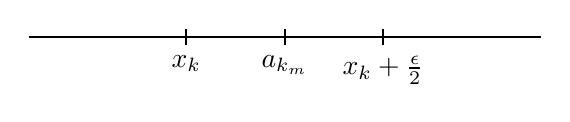
\begin{tikzpicture}[thick]
    \draw(-1,0)--(5.5,0);
    \foreach \x/\xtext in {1/{x_k},2.25/{a_{k_m}},3.5/{x_k + \frac{\epsilon}{2}}}
      \draw(\x,3pt)--(\x,-3pt) node[below] {$\xtext$};
  \end{tikzpicture}
\newline
\(\Rightarrow \abs{a_{k_m} - z} = \abs{a_{k_m} - x_k + x_k - z} \le \abs{a_{k_m} - x_k} + \abs{x_k - z} < \frac{\epsilon}{2} + \frac{\epsilon}{2} = \epsilon \) \\
Also \(\forall \epsilon > 0 \exists N \in \N \forall k \ge N\exists a_{k_m} \in (a_n) \quad \abs{a_{k_m} - z} < \epsilon \)
d.h. die Teilfolge \((a_{k_m})_{m\ge 0}\) ist konvergent gegen \(z\)\\
Also \((a_{k_m})\) ist eine konvergente Teilfloge von der beschränkten Folge \((a_n)\).
\end{enumerate}
\end{proof}
\end{satz}

\begin{bem}
Der Satz von Bolzano-Weierstraß ist äquivalent zum Vollstaändigkeitsaxiom.\\
Äquivalente Formulierungen:\\
\begin{itemize}
\item Jede beschränkte Folge reeller Zahlen hat mindestens einen Häufungspunkt
\item Jede beschränkte Folge reeller Zahlen hat einen größten und einen kleinsten Häufungspunkt
\end{itemize}
\end{bem}

\begin{defi}[Cauchy-Folge] 
Eine Folge \((a_n)_{n \ge 0}\) heißt CAUCHY-Folge, wenn gilt:
\[\forall \epsilon > 0 \sp \exists N \in \N \forall n, m \ge N \abs{a_n - a_m} < \epsilon\]
\end{defi}

\begin{satz}
Folgende Aussagen sind äquivalent
\begin{enumerate}
\item Die Folge \((a_n)\) ist konvergent
\item Die Folge \((a_n)\) ist eine Cauchy-Folge
\end{enumerate}
\begin{proof}
\(1) \Rightarrow 2) \) \\
Sei \(\liminf{a_n} = a \Rightarrow \forall \epsilon > 0 \sp \exists N \sp \forall m \ge N \abs{a_n a} < \frac{\epsilon}{2} \Rightarrow \forall n, m \ge N \\
\abs{a_n - a_m} = \abs{a_n - a + a - a_m} \le \abs{a_n - a }  + \abs{a_m - a} <  \frac{\epsilon}{2}+ \frac{\epsilon}{2} = \epsilon \\
\Rightarrow a_n\) ist eine Cauchy Folge\\
\(2) \Rightarrow 1) \) \\
Jede Cauchy Folge ist beschränkt. Sei \(\epsilon = 1 \Rightarrow \exists N \in N \sp \forall n, m \ge N \abs{a_n - a_m} < 1 \Rightarrow \abs{a_n - a_N} < 1 \\
\Rightarrow \abs{a_n} = \abs{a_n - a_N + a_N} \le \abs{a_n - a_N} + \abs{a_N} < 1 + \abs{a_N} \forall n  \ge N\\
\Rightarrow \forall n \in \N \sp \abs{a_n} \le max\{\abs{a_0},\dots,\abs{a_{N-1}},\abs{a_N} + 1\} \Rightarrow (a_n)\) ist beschränkt.\\
Nach dem Satz von Bolzano-Weierstraß existiert eine konvergente Teilfolge \((a_{n_k})_{k \ge 0} \text{ sei } \liminf[k]{a_{n_k}} = a\).\\
Wir zeigen. \(\liminf{a_n} = a.\)\\
Sei \(\epsilon > 0\). Wähle \(m\) so groß, dass \(\abs{a_m - a_n} < \frac{\epsilon}{2} \forall n,m \ge N \text{ und } \abs{a_{n_k} - a} < \frac{\epsilon}{2} \sp \forall k \ge N\\
\Rightarrow \abs{a-a_n} = \frac{a - a_{n_k} + a_{n_k} - a_n} \le \abs{a- a_{n_k}} + \abs{a_{n_k} - a_n} < \frac{\epsilon}{2} + \frac{\epsilon}{2} = \epsilon \text{, da } n_k \ge n \ge N\)
\end{proof}
\end{satz}

%% KORRIGIERE AB HIER!
\begin{bsp}[Verfahren zur Berechnung der Quadratwurzel]
Seien \(a = 0\), \(a_0 > 0\) reelle Zahlen. Wir definieren die Folge \((x_n)\) rekursiv.
\begin{align*}
x_0 = x_0
x_{n+1} = \frac{1}{2}\left(x_n + \frac{a}{x_n}\right)
\end{align*}
Wir zeigen: \((x_n)\) ist konvergent und \(\liminf{x_n} = x \text{ und } x^2 = a\).
\begin{proof}
\begin{enumerate}
\item \(x_n > 0 \forall n \ge 0\) \\
IA{n=0} \( x_0 > 0 \) \\
IV \(x_{n+1} =  \frac{1}{2}\left(x_n + \frac{a}{x_n}\right)\) \\
IS{n $\mapsto$ n+1}
Sei \(x_n > 0 \Rightarrow x_{n+1} = \underbrace{\frac{1}{2}}_{> 0}\left(\underbrace{x_n}_{> 0} + \underbrace{\overbrace{\frac{a}{x_n}}^{> 0}}_{>0}\right) > 0\) \\
\(\Rightarrow (x_n) \) ist nach unten durch \(0\) beschränkt.
\item \(x_n^2 \ge a \quad \forall n \ge 1\) \\
denn \(x_{n+1}^2 - a = \frac{1}{4}\left(x_n + \frac{a}{x_n}\right)^2  - a = ... a in klammer rein zieihen und ausrechnen ... = \frac{1}{4} (mals a quradrat) \ge 0\)
\item \((x_n)\) ist monoton fallend \\
\(x_n - x_{n+1} = x_n - \frac{1}{2} \left(x_n + \frac{a}{x_n}\right) = (x_n in klammer rein zeihen und ausrehcnen ) = \frac{1}{(2x_n)(x_n^2 - a)} \ge 0 \\
 weil beides \ge 0 (x_n > 0) \Rightarrow x_>n >= x_{n+1} \) \\
Nach dem Monotonie-Kriterium ist \((x_n)\) konvergent.
\item Sei \(x= \liminf{x_n} \Rightarrow x = \liminf{x_{n+1}} = \liminf{\frac{1}{2}\left(x_n + \frac{a}{x_n}\right)} = \frac{1}{2}\left(\liminf{x_n} + \frac{a}{\liminf{x_n}}\right) =  \frac{1}{2}\left(x + \frac{a}{x}\right) \Rightarrow 2x = x + \frac{a}{x} \Rightarrow  \\
x = \frac{a}{x} \Rightarrow x^2 = a\).
\end{enumerate}
\end{proof}
\end{bsp}
Die positive Lösung der Gleichung \(x^2 = a\) heißt die Quadratwurzeln von \(a\). Wir Schreiben \(x = \sqrt{a}\).

\subsection{Reihen}

\begin{defi}
Sei \((a_n)_{n \ge 0}\) eine Folge reeller Zahlen. Sei weiters \(S_N = \sum_{n = 0}^{N}{a_n} \text{ die }N\)-te Partialsumme, dann heißt die Folge \((S_N)_{N \ge 0}\) der Partialsummen eine unendliche Reihe.\\
\[\text{Schreibweise: }\suminf{a_n}\]
Konvergiert die Folge \((S_N)\text{ mit }\liminf{S_N} = s \text{, dann heißt } \suminf{a_n} = s\) der Wert der Reihe.Man sagt: Die Reihe \(\suminf{a_n}\) konvergiert.
\[\text{Schreibweise: } \suminf{a_n} < \infty\].
\end{defi}

\begin{bsp}
\begin{enumerate}
\item Die geometrische Reihe. Sei \(\abs{a} < 1 \Rightarrow \suminf{a^n} = \frac{1}{1-a}\text{. Ist }\abs{a} \ge 1\text{, dann ist }\suminf{a^n}\) divergent.
\begin{proof}
Die geometrische Summe: \(\sum_{n = 0}^{N}{a^n} = \frac{1-a^{N+1}}{1-a}\) dann:
\begin{math}
IA{N=0} 1 = a^0 = (1-a) / (1- a) = 1\\
IV \sum_{n = 0}^{N}{a^n} = \frac{1-a^{N+1}}{1-a}\\
IS{N \mapsto N+1}\\
\sum_{n = 0}^{N+1}{a^n} = a^{N+1} + \sum_{n = 0}^{N}{a^n} \overset{IV}{=} a^{N+1} + \frac{1-a^{N+1}}{1-a} = .... \text{selber} \\ %todo
\text{Sei }S_N = \sum_{n=0}^{N}{a^n} = \frac{1 - a^{N+1}}{1- a} \\
\text{Sei }\abs{a} < 1\text{. Dann folgt }\liminf{a^N} = 0 \\
\Rightarrow \liminf{S_N} = \liminf{\frac{1-a^{N+1}}{1-a}} = \frac{1}{1-a}\\
\text{Sei }a \ge 1 \Rightarrow \sum_{n=0}^{N}{a^n} \ge \sum_{n=0}^{N}{1} = N+1 \longrightarrow \inf \\
\text{Sei }a \le -1 \Rightarrow a = -b \text{ mit }b \ge 1 \Rightarrow \sum_{n=0}^{N}{a^n} \ge \sum_{n=0}^{N}{(-1)^nb^n} \text{ divergent}
\end{math}
\end{proof}
\item Die harmonische Reihe: \(\sum{n=1}{\infty}{\frac{1}{n}} = +\infty\)
\begin{proof}
\begin{math}
S_{2^N} = \sum_{n = 1}^{2^N}{\frac{1}{n}} = 1 +\underbrace{\frac{1}{2}}_{=\frac{1}{2}} + \underbrace{\frac{1}{3} + \frac{1}{4}}_{=\frac{1}{2}} + \underbrace{\frac{1}{5} + \frac{1}{6} + \frac{1}{7} + \frac{1}{8}}_{=\frac{1}{2}} + \underbrace{\frac{1}{9} + ... + \frac{1}{16}}_{=\frac{1}{2}} + \underbrace{\frac{1}{17} + ..... + }_{=\frac{1}{2}} + \underbrace{\frac{1}{2^{N-1}+1}+ .... + \frac{1}{2^N}}_{=\frac{1}{2}} \ge 1 + n \frac{1}{2} > \frac{n}{2} \longrightarrow +\infty
\end{math}
Würde \((S_N)_{N\ge1}\) konvergieren, dann auch die Teilfolge \((S_{2^N})_{N \ge 1}\), da diese dievergiert, divergiert auch \((S_N)_N\)
\end{proof}
\item $ \Suminf{(\frac{1}{n(n+1)}}= 1 $
\begin{proof}
\begin{math}
S_N = \sum_{n=1}^{N}{\frac{1}{n(n+1)}} = \sum_{n=1}^{N}{\frac{1}{n}} - \frac{1}{n+1} = \sum_{n=1}^{N}{\frac{1}{n}} - \sum_{n=1}^{N}{\frac{1}{n+1}} = 1+ \sum_{n=2}^{N}{\frac{1}{n}} - \sum_{n=2}^{N+1}{\frac{1}{n}} = 1+ \sum_{n=2}^{N}{\frac{1}{n}} - \sum_{n=2}^{N}{\frac{1}{n}} + \frac{1}{N+1} = 1 + \frac{1}{N+1} \longrightarrow 1
\end{math}
\end{proof}
\end{enumerate}
\end{bsp}

\begin{satz}
Seien \suminf{a_n} und \suminf{b_n} zwei konvergente Reihen und \(\lambda \in \R\)
Dann ist auch \(\suminf{\lambda a_n + b_n}\) konvergent und \( \suminf{\lambda a_n + b_n} = \lambda \suminf{a_n} + \suminf{b_n}\)
\begin{proof} folgt auf grund der Rechenregeln für konvergente Folgen.\end{proof}
\end{satz}

\begin{satz}[Cauchy-Kriterium für Reihen]
Die Reihe \(\suminf[k]{a_k}\) ist konvergent, genau dann wenn gilt:
\[\forall \epsilon > 0 \sp \exists N(\epsilon) \in \N \quad \forall n \ge m \ge N \qquad \abs{\sum_{k=m}^{n}{a_k}} < \epsilon \qquad (\star)\]
\begin{proof}
\(S_n - Sm = \sum_{k=0}^{n}{a_k} - \sum{k=0}{m}{a_k} = \sum_{k=m}^{n}{a_k}\). \((\star)\) bedeutet die \((S_n)_n\) ist eine Cauchy-Folge \(\Leftrightarrow (S_n)_n\) ist konvergent
\end{proof}
\end{satz}

\begin{korr}
Ist \suminf[k]{a_k} konvergent \(\Rightarrow \liminf[k]{a_k} = 0\).
\begin{proof}
\(a_n = \sum{k = m}{n}{a_k}\text{. Da } \suminf[k]{a_k} < \infty \overset{\Rightarrow}{\text{Cauchy-Kriterium}} \forall \epsilon > 0 \sp \exists N \in \N \quad \forall n \ge N \abs{a_N} = \abs{ \sum{k = m}{n}{a_k}} < \epsilon  \Rightarrow \liminf{a_n} = 0\)
\end{proof}
\end{korr}

\begin{bem}
Die Umkehrung des Korrolars gilt nicht. z.B. \(\liminf{1/n} = 0\text{ aber }\suminf{1/n} = \infty \) harmonische Reihe.
\end{bem}

\begin{defi}
Die Reihe \suminf[k]{a_k} heißt absolut konvergent, wenn wenn die Reihe \suminf[k]{\abs{a_k}} konvergiert.
\end{defi}

\begin{satz}
Jede absolut konvergente Reihe ist auch konvergent.
\begin{proof}
\begin{math}
\text{Sei }\suminf[k]{\abs{a_k}} < \infty  \overset{\Rightarrow}{\text{Cauchy-Kriterium}} \forall \epsilon > 0 \sp \exists N \in \N \quad \forall n \ge m \ge N \quad \abs{\sum{k=m}{n}{\abs{a_k}}} < \epsilon \overset{\Rightarrow}{\text{Dreiecksungleichung}} \abs{\sum{k=m}{n}{a_k}} \le \abs{\sum{k=m}{n}{\abs{a_k}}} < \epsilon \forall n \ge m \ge N
\overset{\Rightarrow}{\text{Cauchy-Kriterium}} \suminf[k]{a_k}\text{ ist konvergent.}
\end{math}
\end{proof}
\end{satz}

\begin{bem}
Die Umkehrung des Satzes gilt nicht. zB kann man zeigen, dass die Reihe \(\suminf[k]{(-1)^k\frac{1}{k}}\) konvergiert. Aber die Reihe \(\suminf[k]{\abs{(-1)^k\frac{1}{k}}} = \suminf[k]{\frac{1}{k}} = \infty\)
\end{bem}

\begin{satz}[Majoranten-Kriterium]
Sei \suminf[k]{b_k} konvergent mit \(b_k \ge 0 \forall k \ge N_0\).
Sei \((a_k)_{k=0}^{\infty}\) eine Folge mit \(\abs{a_k} \le b_k  \forall k \ge N_0 \Rightarrow \suminf[k]{a_k}\) ist absolut konvergent.
\begin{proof}
\begin{math}
\text{Sei }\suminf[k]{b_k} < \infty \text{ und } b_k > 0 \overset{\Rightarrow}{\text{Cauchy-Kriterium}} \forall \epsilon > 0 \sp \exists N \in \N \quad \forall n \ge m \ge N \quad \abs{\sum{k=m}{n}{b_k}} < \epsilon \overset{\Rightarrow}{\abs{a_k} \le b_k} \abs{\sum{k=m}{n}{\abs{a_k}}} \le \abs{\sum{k=m}{n}{b_k}} < \epsilon \forall n \ge m \ge N
\overset{\Rightarrow}{\text{Cauchy-Kriterium}} \suminf[k]{\abs{a_k}} \text{ ist konvergent. }\Rightarrow \suminf[k]{a_k}\text{ ist absolut konvergent.}
\end{math}
\end{proof}
\end{satz}

\begin{korr}[Minoranten-Kriterium]
Sei \suminf[k]{b_k} divergent mit $b_k \ge 0 \forall k \ge N_0$.
und $(a_k)_{k=0}^{\infty}$ eine Folge mit $\abs{a_k} \ge b_k  \forall k \ge N_0
\Rightarrow \suminf[k]{a_k}$ ist auch divergent.
\begin{proof}
Wäre \(\suminf[k]{a_k}\) konvergent, dann wäre nach dem Majoranten-Kriterium \(\suminf[k]{b_k}\) konvergent, da \(\abs{b_k} \le a_k\). \WSP
\end{proof}
\end{korr}

\begin{satz}[Quotienten-Kriterium]
Sei \suminf{a_n} eine Reihe mit \(a_n \ne 0 \forall n \ge n_0\)
Existiert eine reelle Zahl \(q \text{ mit } 0 < q < 1 \text{ sodass }\abs{\frac{a_{n+1}}{a_n}} \le q < 1 \forall n \ge n_0
\Rightarrow \suminf{a_n}\) ist absolut konvergent.
\begin{proof}
\begin{math}
\text{Sei } \abs{\frac{a_{n+1}}{a_n}} \le q < 1  \forall n \ge 0 \text{(o.B.d.A.)} \Rightarrow \abs{a_{n+1}} \le q \abs{a_n} \Rightarrow \abs{a_n} \le q\abs{a_{n-1}} \le q^2 \abs{a_{n-2}} \le ... \le q^n \abs{a_0}.
\text{Also }\abs{a_n} \le q^n \abs{a_0}, da \suminf{\abs{a_n}} \le \suminf{q^n \abs{a_0}} = \abs{a_0} \suminf{q^n} = \abs{a_0} \frac{1}{1-q} \text{, denn } 0 < q < 1\text{, geometrische Reihe.}
\Rightarrow \text{ aus dem Majoranten-Kriterium folgt \suminf{a_n} ist absolut konvergent.}
\end{math}
\end{proof}
\end{satz}

\begin{korr}[einfaches Quotienten-Kriterium]
Sei \(a_n \ne 0 \sp \fa n > n_0\) und existiert \(\liminf{\abs{\frac{a_n+1}{a_n}}}\text{ und ist }\liminf{\abs{\frac{a_n+1}{a_n}}} < 1
\Rightarrow \suminf{a_n}\) ist absolut konvergent.
\begin{proof}
\begin{math}
\text{Sei } \liminf{\abs{\frac{a_n+1}{a_n}}} = \alpha < 1 \\
\text{Sei } \epsilon = \frac{1 - \alpha}{2} > 0 \Rightarrow \exists N \sp \forall n \ge N \quad \abs{\abs{\frac{a_{n+1}}{a_n}} - \alpha} < \epsilon  = \frac{1-\alpha}{2}
\Rightarrow \abs{\frac{a_(n+1)}{a_n}} < \frac{1-\alpha}{2} + \alpha = \frac{1+\alpha}{2} \overset{<}{\text{da } \alpha < 1} 1+\frac{1}{2} = 1
\text{Sei } q = \frac{1 + \alpha}{2} < 1 und \abs{\frac{a_(n+1)}{a_n}} < q < 1
\end{math}
Nach dem Quotienten-Kriterium ist \suminf{a_n} absolut konvergent
\end{proof}
\end{korr}

\begin{bsp}
\begin{enumerate}
\item \(\suminf{\frac{1}{n^k}} < \infty \qquad \forall k \ge 2 \) 
[Bemerkung: Die Konvergenz gilt auch \(\fa k \in \R, k > 1\) ohne Beweis]
\begin{proof}
\begin{math}
\frac{1}{n^k} \le \frac{1}{n^2} \qquad \forall k \ge 2 \text{ und }\\
\frac{1}{n^2} \le \frac{2}{n(n+1)} \text{, denn }\Leftrightarrow 2n^2 \ge n(n+1) \Leftrightarrow n^2 \ge n \Leftrightarrow n \ge 1 \\ 
\Rightarrow \frac{1}{n^k} \le \frac{2}{n(n+1)} \forall k \ge 2 \text{ und } \\ 
\suminf{\frac{2}{n(n+1)}} = 2 \suminf{\frac{1}{n(n+1)}} = 2 * 1 = 2 \overset{\Rightarrow}{Majoranten-Kriterium} \suminf{\text{1}{n^k}} < \infty \forall k \ge 2
\end{math}
Frage: Wie sind die Werte der Reihe \(\suminf{1/n^k} \text{ für } k \ge 2 \)
Euler: \(\suminf{\frac{1}{n^2}} = \frac{\pi^2}{6} \text{, } \suminf{\frac{1}{n^4}} = \frac{\pi^4}{90} \text{, \dots , } \suminf{\frac{1}{n^{2k}}} = C_k \pi^{2k}\)
Aber: \(\suminf{\frac{1}{n^3}} \in \R \setminus \Q \text{, } \suminf{\frac{1}{n^5}} = ? \text{, \dots , } \suminf{\frac{1}{n^{2k+1}}} = ?\)
\end{proof}
\item Die Reihe \suminf{\frac{n^2}{2^n}} ist konvergent.
\begin{proof}[Quotienten-Kriterium]
\(\abs{\frac{a_{n+1}}{a_n}} = \frac{\frac{(n+1)^2}{2^{n+1}}}{\frac{n^2}{2^n}} = \frac{2^n(n+1)^2}{2^{n+1}n^2} = \frac{1}{2} * \left(\frac{n+1}{n}\right)^2 = \frac{1}{2} \left(\frac{1}{1+\frac{1}{n}}\right)^2 \longrightarrow \frac{1}{2} < 1\)
\end{proof}
\item Die Exponentialfunktion Die Reihe $\suminf[k]{\frac{x^k}{k!}}$ ist für jedes $x \in \R$ absolut konvergent
\begin{proof}[Quotienten-Kriterium]
\(\abs{\frac{a_{k+1}}{a_k}} = \abs{\frac{\frac{x^{k+1}}{(k+1)!}}{\frac{x^k}{k!}}} = \frac{\abs{x^{k+1}} * k!}{\abs{x^k} * (k+1)!} = \frac{\abs{x}}{k+1} \overset{\longrightarrow}{k \to \infty} 0 \sp \forall x \in \R\\
\Rightarrow \suminf[k]{\frac{x^k}{k!}}\) ist absolut konvergent.
\end{proof}
\end{enumerate}
\end{bsp}

\begin{bem}
\begin{enumerate}
\item Für \(k = 1\) ist die harmonische Reihe \suminf{\frac{1}{n}} divergent.
\item Das Quotienten-Kriterium ist hier nicht anwendbar, denn \\
\[\suminf{\frac{1}{n}} \qquad \frac{a_{n+1}}{a_n} = \frac{1}{1 + \frac{1}{n}} \longtoinf{n} 1 \not < 1\]
\[\suminf{\frac{1}{n^2}} \qquad \frac{a_{n+1}}{a_n} = \left(\frac{1}{1 + \frac{1}{n}}\right)^2 \longrightarrow 1 \not < 1\]
\end{enumerate}
\end{bem}

\begin{defi}
Die Funktion \(exp: \R \to \R \text{ mit } exp(x) \mapsto \e^x = \suminf{\frac{x^n}{n!}}\) heißt Exponentialfunktion.\\
Die Zahl \(\e = exp(1) = \suminf{\frac{1^n}{n!}} \) heißt Euler'sche Zahl.
\end{defi}

\begin{bem}
Wir werden später zeigen:
\[\e = \frac{1^n}{n!} = \liminf{\left(1 + \frac{1}{n}\right)^n} \approx 2,71828...\]
\end{bem}




 






















%soll am ende stehen7
\newpage
\section{Test}
zum Formeln raus kopieren
\begin{enumerate}
\item \(\to\)
\item $(a_n)$
\item \(\liminf{a_n}\)
\item \(\suminf{a_n}\)
\item \longtoinf
\end{enumerate}
\[\liminf{a_n}\]
\[\sum_{n = 0}^{\infty}{a_n}\]
\[\Sum{n}{k}\]

Verschiedene Größen:
\begin{enumerate}
\item $\displaystyle \suminf[n]{a_{n_k} + \frac{b_n}{c_n}}$	
\item $\textstyle \suminf[n]{a_{n_k} + \frac{b_n}{c_n}}$	
\item $\scriptstyle \suminf[n]{a_{n_k} + \frac{b_n}{c_n}}$	
\item$\scriptscriptstyle \suminf[n]{a_{n_k} + \frac{b_n}{c_n}}$	
\end{enumerate}

\begin{proof}
\IA \\
\IV \\
\IS \\
\end{proof}

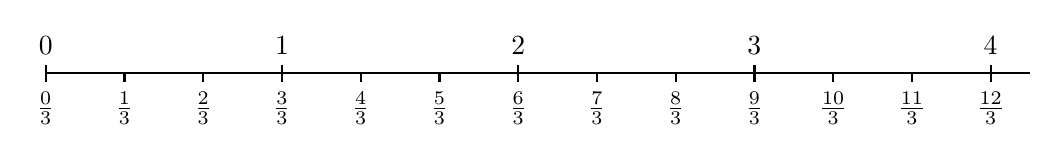
\begin{tikzpicture}[thick]
\newline
    \draw(0,0)--(12.5,0);
    \foreach \x/\xtext in {0/0,3/1,6/2,9/3,12/4}
      \draw(\x,0pt)--(\x,3pt) node[above] {\xtext};
    \foreach \x in {0,1,...,12}
      \draw(\x,0pt)--(\x,-3pt) node[below] {$\frac{\x}{3}$};
  \end{tikzpicture}


\begin{center}
\begin{tikzpicture}
        \draw[step=1,help lines,black!0] (-1,-1) grid (4,4);
        \draw[->] (-0.5,0) -- (3.5,0)  node[below right] {$Re(z)$};
        \draw[->] (0,-0.5) -- (0,3.5)  node[above left]{$Im(z)$};
        \foreach \Point/\PointLabel in {(0,1)/{\im}, (1,0)/1, (2.21,1.75)/{z=(a,b)}}
        \draw[fill=black] \Point circle (0.05) node[above right] {$\PointLabel$};
        \foreach \Point/\PointLabel in {(2.21,0)/a, (0,1.75)/b}
        \draw \Point circle (0.05) node[above right] {$\PointLabel$};
\end{tikzpicture}
\end{center}

 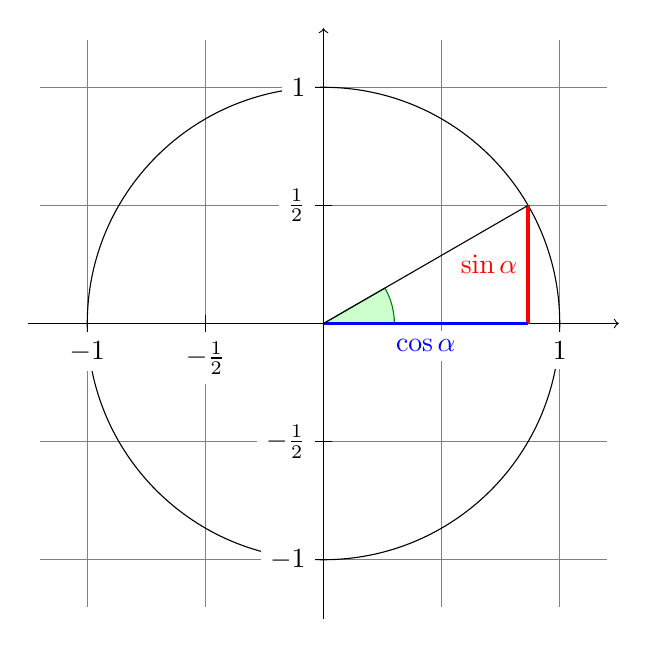
\begin{tikzpicture}[scale=3]
 \draw[step=.5cm, gray, very thin] (-1.2,-1.2) grid (1.2,1.2); 
 \filldraw[fill=green!20,draw=green!50!black] (0,0) -- (3mm,0mm) arc (0:30:3mm) -- cycle; 
 \draw[->] (-1.25,0) -- (1.25,0) coordinate (x axis);
 \draw[->] (0,-1.25) -- (0,1.25) coordinate (y axis);
 \draw (0,0) circle (1cm);
 \draw[very thick,red] (30:1cm) -- node[left,fill=white] {$\sin \alpha$} (30:1cm |- x axis);
 \draw[very thick,blue] (30:1cm |- x axis) -- node[below=2pt,fill=white] {$\cos \alpha$} (0,0);
 \draw (0,0) -- (30:1cm);
 \foreach \x/\xtext in {-1, -0.5/-\frac{1}{2}, 1} 
   \draw (\x cm,1pt) -- (\x cm,-1pt) node[anchor=north,fill=white] {$\xtext$};
 \foreach \y/\ytext in {-1, -0.5/-\frac{1}{2}, 0.5/\frac{1}{2}, 1} 
   \draw (1pt,\y cm) -- (-1pt,\y cm) node[anchor=east,fill=white] {$\ytext$};
 \end{tikzpicture}


\end{document}
